\section{Обзор предметной области}

\subsection{Постановка задачи}

Задача генерации речи имеет простую математическую формулировку. По заданному отрывку текста со строковым представлением (конечная последовательность символов из конечного алфавита), сгенерировать аудиодорожку с хорошо слышимой человеческой речью соответствующей заданному отрывку. Формат аудио обычно представляет из себя последовательность из 16-битных чисел от $-1.0$ до $1.0$ -- дискретное приближение непрерывной аудиоволны. Основной параметр такого формата - это частота дискретизации, выражаемая в герцах (Гц, Hz). Популярными частотами для аудио отрывков в системах генерации речи являются $22.05$ кГц и $24$ кГц. Чем выше частота дискретизации -- тем лучше качество аудио (так как лучше приближение), но тем сложнее уловить зависимости для генерации (Рисунок~\ref{fig:sample-rate}).

\begin{figure}[!ht]
\centering
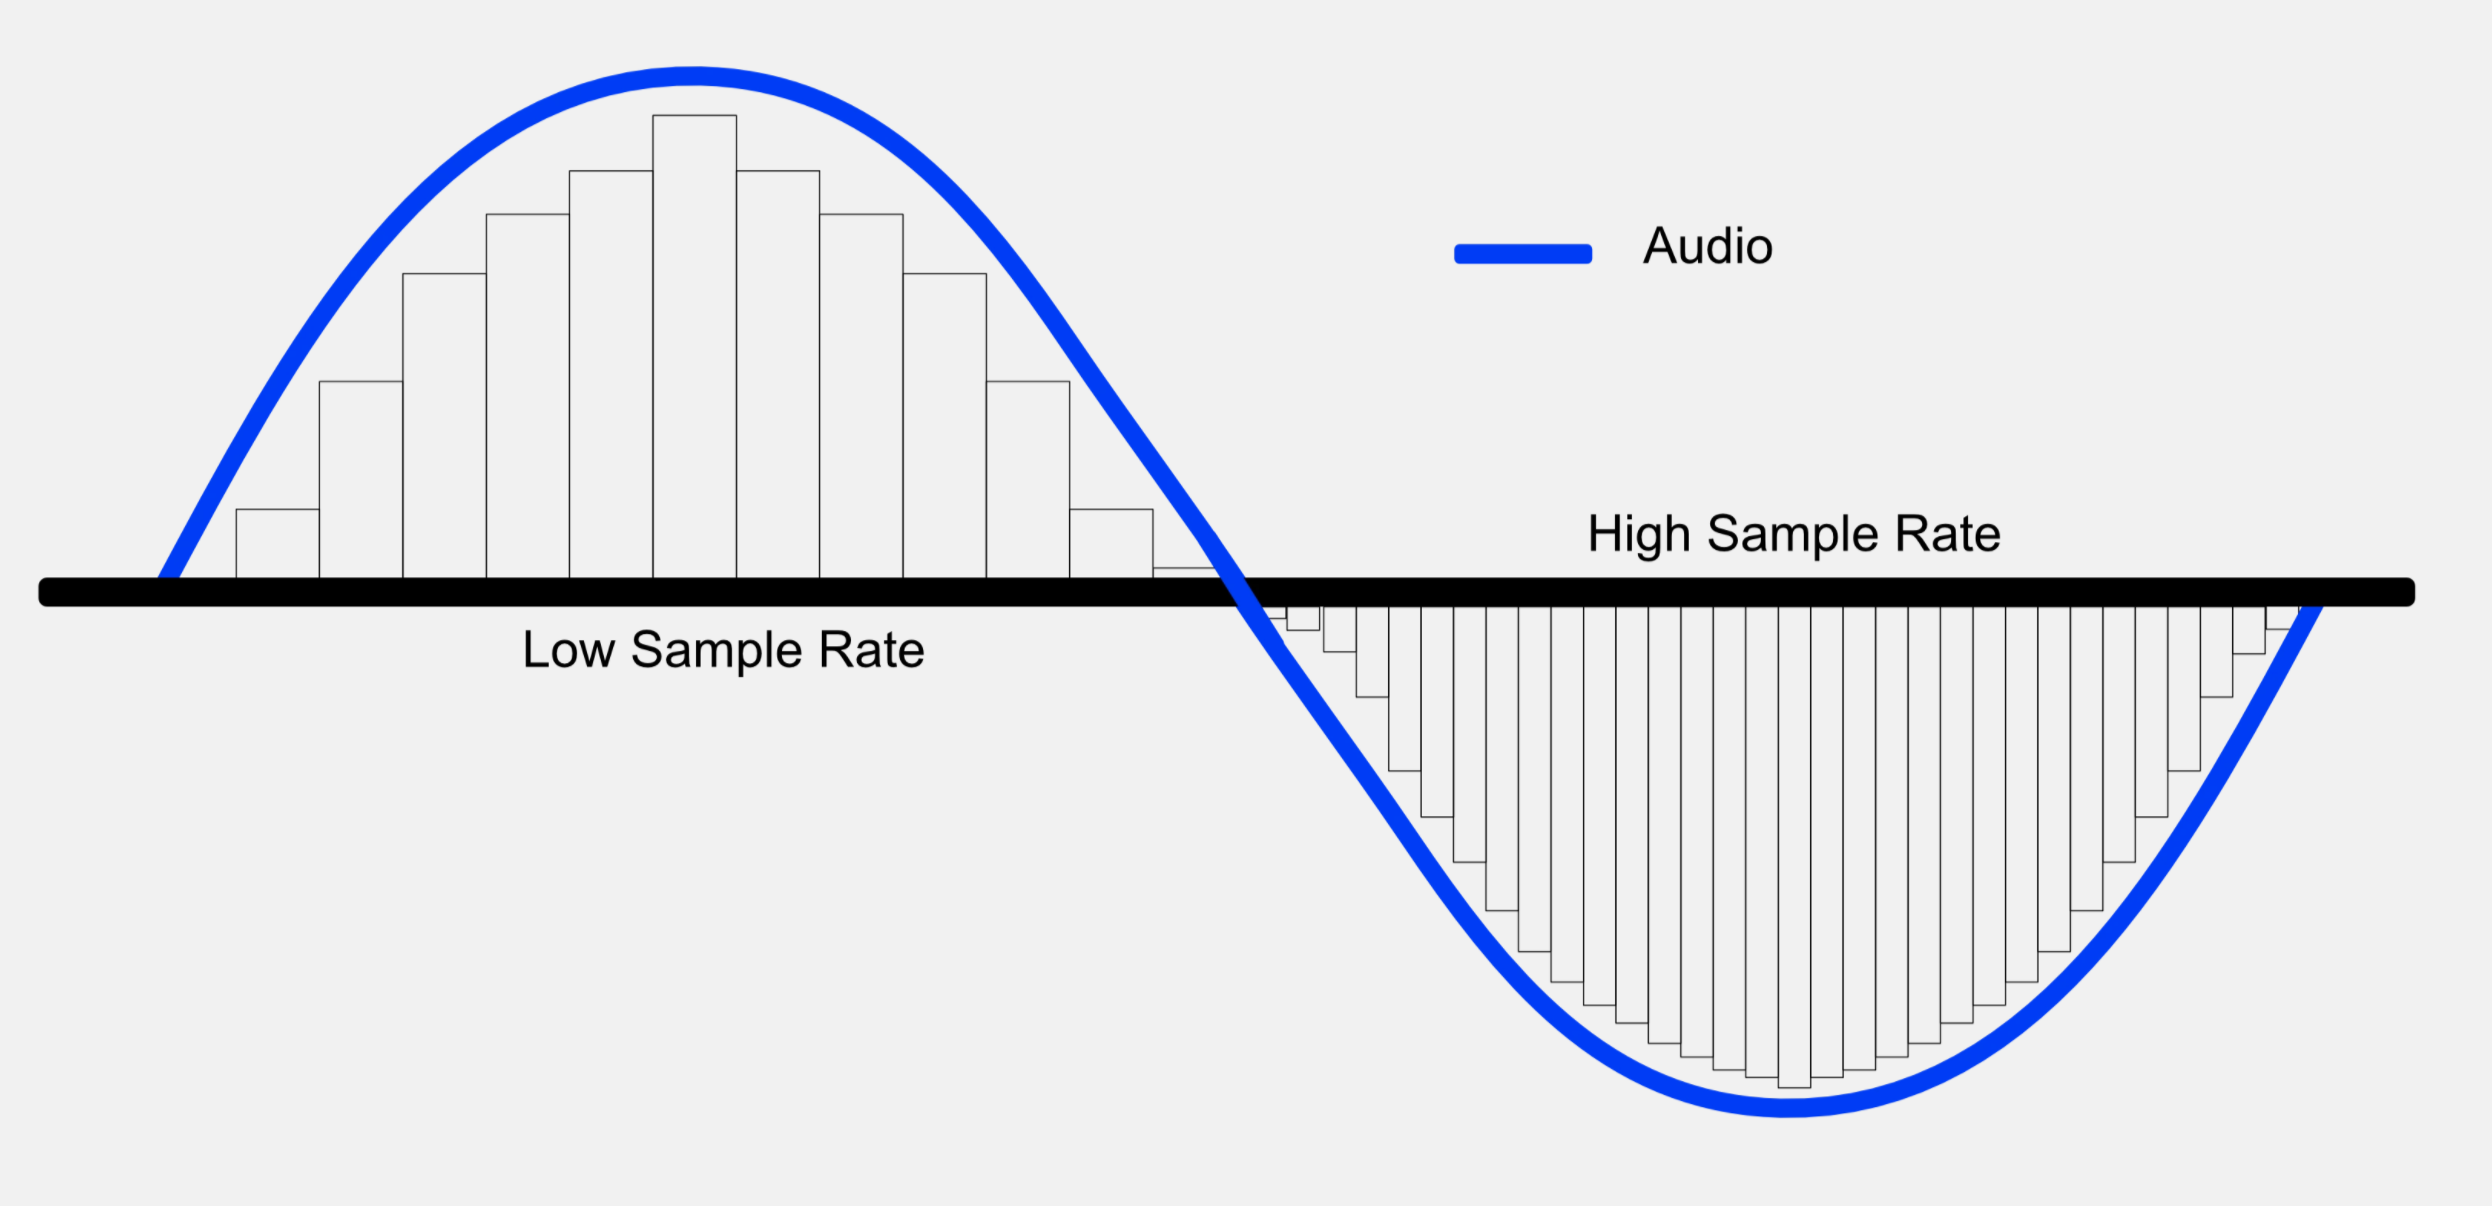
\includegraphics[width=1.0\textwidth]{images/sample-rate.png}
\caption{Примеры различной частота дискретизации (sample rate) для представления аудио}
\label{fig:sample-rate}
\end{figure}

Модели на основе нейронных сетей (NN) для преобразования текста в речь (Text-To-Speech, TTS) превзошли как конкатенативный (concatenative), так и статистический параметрический подходы для синтеза речи с точки зрения качества. Они также значительно упрощают процесс синтеза речи. Традиционно. системы синтеза речи объединяет несколько блоков: модель для извлечения лингвистических признаков из текста, модель длительности, модель предсказания акустических признаков и вокодер на основе обработки сигналов~\cite{taylor}, который служит для преобразования акустических признаков в аудиодорожку. Нейронные TTS системы, как правило, имеют два этапа (Рисунок~\ref{fig:tts-pipeline}). На первом этапе модель генерирует мэл-спектрограммы из текста. На втором этапе вокодер на основе нейронной сети синтезирует речь из мэл-спектрограмм. Большинство моделей TTS на основе NN имеют архитектуру экодер-декодер~\cite{bahdanau} с операциями с механизмом внимания (attention), которая, как было замечено, имеет некоторые общие проблемы:
\begin{enumerate}
    \item A tendency to repeat or skip words~\cite{fastspeech}, due to attention failures when some sub\-sequences are repeated or ignored. To handle this issue, attention-based models use additional mechanisms to encourage monotonic attention \cite{tacotron2,deepvoice3,taigman2017}.
    \item Slow inference relative to parametric models.
    \item No easy way to control prosody nor voice speed, since the length of the generated sequence is automatically determined by the decoder.
\end{enumerate}

\begin{figure}[!ht]
\centering
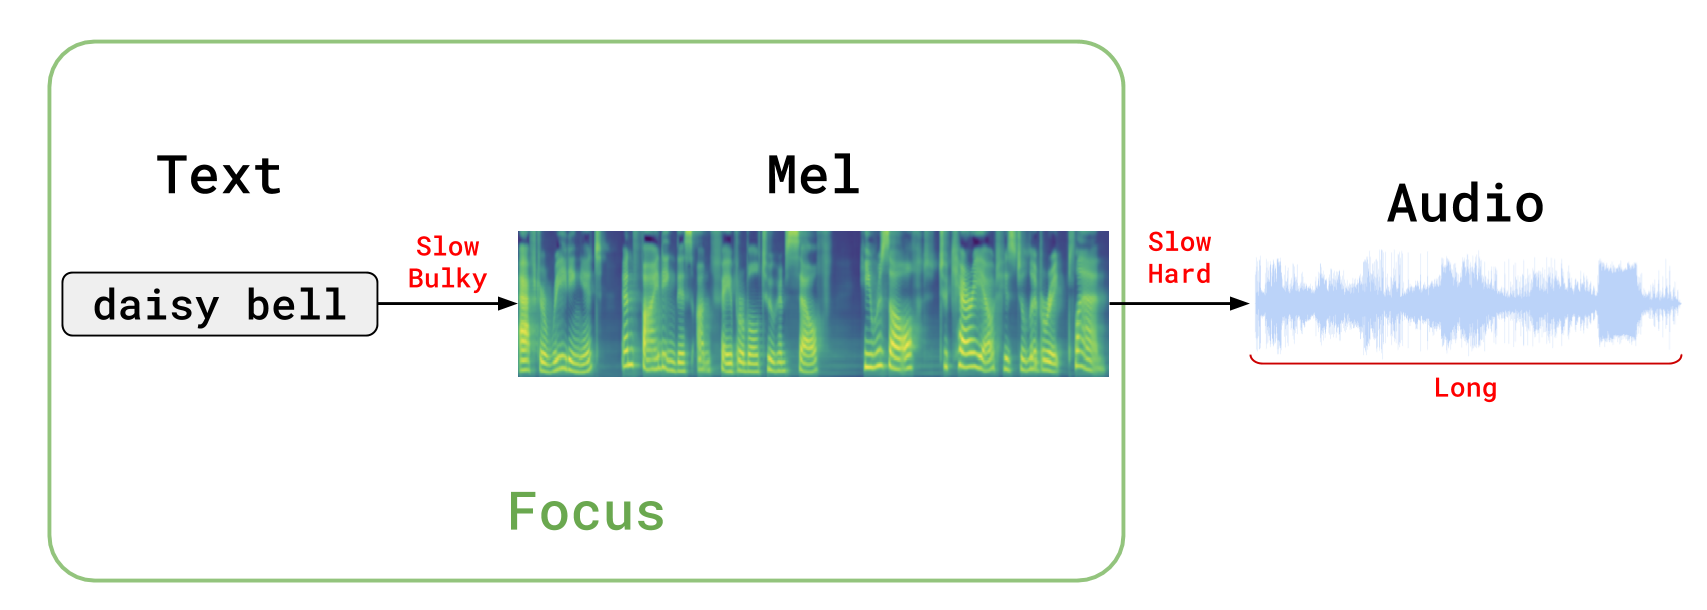
\includegraphics[width=1.0\textwidth]{images/tts-pipeline.png}
\caption{Два шага TTS систем}
\label{fig:tts-pipeline}
\end{figure}

We propose a new neural TTS model to address these three challenges. The model consists of two convolutional networks. The first network predicts grapheme durations. We expand an input text by repeating each symbol according to the predicted duration. The second network generates mel-spectrograms from an expanded text. Finally, we use the WaveGlow~\cite{waveglow} vocoder to synthesize audio from mel-spectrograms (see Figure~\ref{fig:arch}).

To train the grapheme duration predictor, we need the ground truth alignment between input characters and audio. A similar alignment problem exists in automatic speech recog\-nition (ASR) which is addressed by using Connectionist Temporal Classification (CTC). CTC marginalizes over the set of all valid alignments. However, if we take the most likely output at each moment, we can use it for alignment between the input audio and the text output. This alignment is not perfect, and it can have errors. We found that if the ASR model is accurate and has a low character error rate (CER), then we can extract a good-enough alignment between text and audio features. We can use this CTC-based alignment to train the model which will predict grapheme durations for the input text. The explicit grapheme duration predictor replaces attention-based alignment to eliminate word skipping and repeating. Experiments on the LJSpeech dataset show that the speech quality for TalkNet is similar to auto-regressive models.

The convolutional structure of both blocks enables parallel training and inference. This structure enables significantly faster inference, has significantly fewer parameters, and can be trained faster than models with similar quality of generated speech, such as FastSpeech~\cite{fastspeech} and Tacotron 2~\cite{tacotron2}.

\subsection{Обзор методов генерации речи}

A typical statistical parametric TTS pipeline has the following stages: grapheme-to-phoneme conversion, a phoneme duration predictor, an acoustic frame-level feature generator, and a vocoder~\cite{taylor}. Zen et al~\cite{zen-2015,zen-2016} proposed a hybrid NN -- parametric TTS model, where deep neural networks are used to predict the phoneme duration and to generate frame-level acoustic features. The phoneme duration predictor was trained on Hidden Markov Model (HMM)-based phonetic alignments.  

DeepVoice models~\cite{deepvoice1,deepvoice2} also adopt the traditional TTS structure, but they replace all components with NNs. To train the phoneme duration predictor, an auxiliary CTC-based model for phonetic segmentation was used to annotate  data with phoneme boundaries. Tacotron~\cite{tacotron1,tacotron2} is an end-to-end NN which takes characters as input and directly outputs the mel-spectrogram. Tacotron 2 uses an encoder-attention-decoder architecture. The encoder is composed from three convolutional layers plus a single bidirectional LSTM. The decoder is a recurrent neural network (RNN) with location-sensitive monotonic attention.

The sequential nature of RNN-based models limits the training and inference efficiency. There has been a number of TTS models without RNNs. DeepVoice 3~\cite{deepvoice3} replaces an RNN with a fully-convolutional encoder-decoder with monotonic attention. Switching from RNN to a convolutional neural network (CNN) makes training faster, but the model inference is still auto-regressive. Another end-to-end TTS model, which does not use RNNs, is ParaNet~\cite{paranet}. ParaNet is a convolutional encoder-decoder with attention. It distills attention from a teacher auto-regressive TTS model. Lastly, Transformer-TTS~\cite{transformer-tts} replaces an RNN-based encoder-decoder with a Transformer-like  attention-only architecture~\cite{attention-is-all}. Transformer-TTS first converts text to phonemes using a rule-based converter. Using phoneme sequences as input, Transformer-TTS generates mel-spectrograms.  

As with other attention-based models, Tacotron, Transformer-TTS and ParaNet occasionally miss or repeat words~\cite{paranet}. To prevent word skipping and repeating, FastSpeech~\cite{fastspeech} proposes a novel feed-forward Transformer-based model, discarding the conventional encoder-attention-decoder structure. FastSpeech uses an explicit length regulator, which expands the hidden sequence of phonemes according to a predicted duration in order to match the length of a mel-spectrogram sequence. The target phoneme duration is extracted from the attention alignment in an external pre-trained TTS model, Tacotron 2.